\section{Service Requests Workflow}

The lifecycle of a Service Request within the current system is orchestrated through a series of defined states and automated processes, involving interactions between various components and human operators. The flow is designed to manage SRs from initiation to completion, handling approvals, execution, and potential errors.

\begin{figure}[htbp]
    \centering
    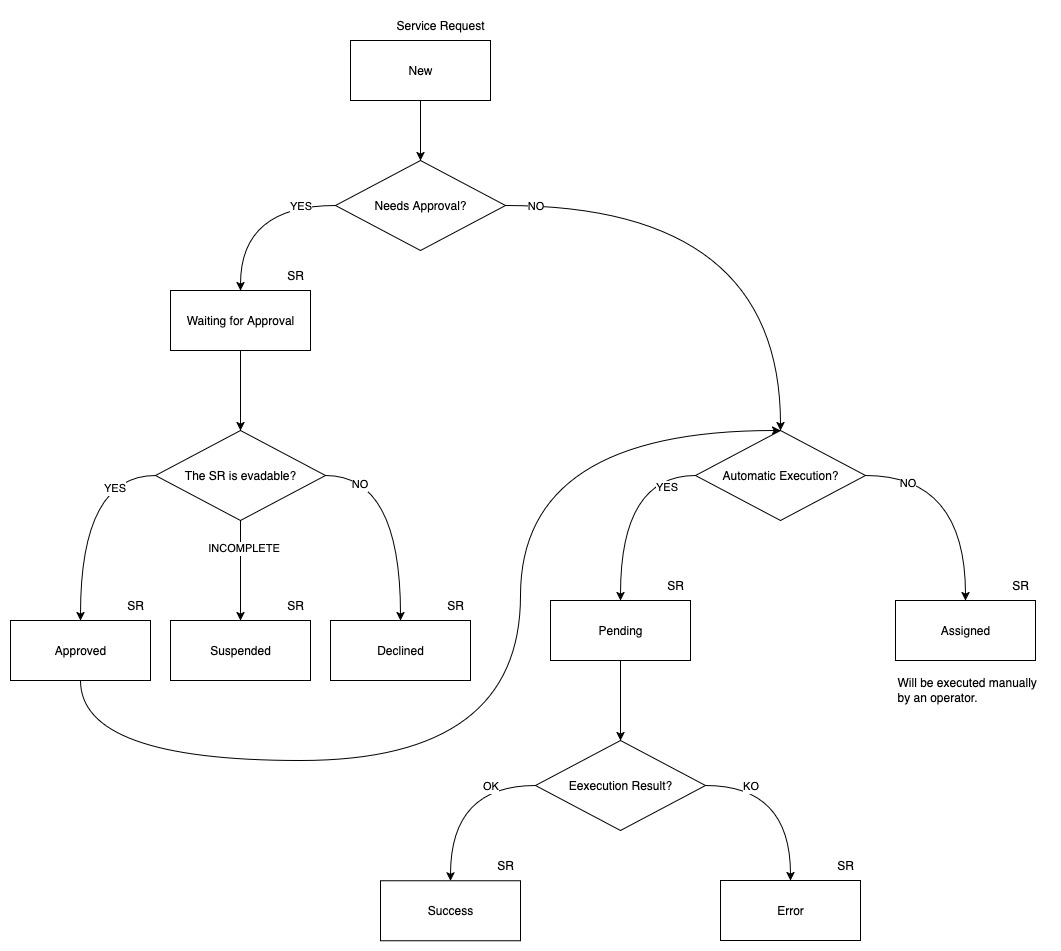
\includegraphics[width=\textwidth,keepaspectratio]{images/sr-state-diagram-simple.jpg}
    \caption{High-Level Service Request Lifecycle}
    \label{fig:sr-state-flowchart-simple}
\end{figure}


In Figure \ref{fig:sr-state-flowchart-simple} a simple and high-level flowchart is shown that illustrates the main flows and scenarios. Instead, in Figure \ref{fig:flowchart-as-is} a complete and detailed flowchart is shown that illustrates all the details about every flow, including information on the jobs and components that manage the various sections of an SR's workflow.

\begin{figure}[htbp]
    \centering
    \includegraphics[height=\textheight, keepaspectratio]{images/as-is/Flowchart AS-IS.jpg}
    \caption{AS-IS Complete Service Request Execution Workflow}
    \label{fig:flowchart-as-is}
\end{figure}

\subsection{SR Initiation and Initial State Management}
A Service Request can be initiated through two primary channels:

\begin{itemize}
    \item \textbf{Via MyElmec Portal}: Clients can submit an SR by completing a dedicated form from the MyElmec portal. Upon saving the form, a ticket is created in the HelpdeskAdvanced (HDA) system with a \texttt{QUALIFIED} status, and a corresponding Service Request is generated in SRP with a \texttt{NEW} status. These two entities are then linked via the HDA Ticket ID;
    \item \textbf{Via HDA Ticket by Elmec Operator}: Operators have the ability to associate a catalog SR directly with a ticket they are managing within the HDA interface. When the ticket is saved in a \texttt{DELEGATED} status, the SR is created in SRP with a \texttt{NEW} status, linked to the ticket, and immediately triggers the SR workflow within SRP.l
\end{itemize}

Following its creation, the system evaluates whether the Service Request requires approval by the operators. The logic for setting the initial SR and HDA ticket states is as follows:
\begin{itemize}
    \item \textbf{If approval is required}: the Service Request is set to \texttt{WAITING FOR APPROVAL} status, and the corresponding HDA ticket is set to \texttt{QUALIFIED}. A communication is added to the ticket, indicating that the SR needs validation from an operator before execution;
    \item \textbf{If no approval is required and it's linked to an automatism}: the Service Request enters a \texttt{PENDING} state, and the HDA ticket is set to \texttt{DELEGATED};
    \item \textbf{If no approval is required and it's not linked to an automatism}: the Service Request is \texttt{ASSIGNED}, and the HDA ticket is set to \texttt{PASSED}. A communication is added to the ticket, noting that the SR requires manual processing by an operator.
\end{itemize}

\subsection{Approval and Execution Workflows}
For SRs requiring approval (\texttt{WAITING FOR APPROVAL} state with an HDA \texttt{QUALIFIED} ticket), an operator's intervention is necessary to validate the request. The operator has three possible actions:
\begin{itemize}
    \item \textbf{Cancel the SR}: the HDA ticket is set to \texttt{CLOSED ABORTED}, the SR status becomes \texttt{DECLINED}, and a notification email is sent to the requesting client;
    \item \textbf{Request client modification}: the HDA ticket is set to \texttt{WAITING USER}, the SR status becomes \texttt{SUSPENDED}, and a notification email is sent to the client. The workflow pauses until the client modifies the SR via Elmec.com;
    \item \textbf{Approve the SR}: the HDA ticket is set to \texttt{DELEGATED}, and the SR status becomes \texttt{APPROVED}.
\end{itemize}

Once a SR is \texttt{APPROVED}, SRP manages its subsequent flow based on whether it is linked to an automatism:
\begin{itemize}
    \item \textbf{If the SR is linked to an automatism}: the SR transitions to a \texttt{PENDING} state, while the HDA ticket remains \texttt{DELEGATED}. This implies it's awaiting automated execution;
    \item \textbf{If the SR is not linked to an automatism}: the SR is immediately set to \texttt{ASSIGNED}, and the HDA ticket is moved to \texttt{PASSED}. A note is added to the ticket indicating that the SR requires manual processing.
\end{itemize}

An SR in \texttt{PENDING} state is awaiting the execution of its associated automatism. The outcome of this automated execution determines the next state:
\begin{itemize}
    \item \textbf{Successful execution}: the SR is set to \texttt{COMPLETED}, and the corresponding HDA ticket is set to \texttt{SOLVED};
    \item \textbf{Unsuccessful execution}: the SR transitions to an \texttt{ERROR} state, and the HDA ticket is set to \texttt{PASSED}. Communication regarding the error is added to the ticket for visibility within HDA.
\end{itemize}

The execution of Service Requests themselves can involve the SRP Agent on the client's Domain Controller for operations requiring client-side interaction (e.g., Active Directory or Exchange environment changes). The SRP Agent periodically checks \texttt{ELMEC-SRP01} for pending SRs. If found, it retrieves the SR details, loads the relevant PowerShell script, and executes it. The agent then informs ELMEC-SRP01 that the SR is running. Monitoring is performed by a scheduled READLOG task on the client side, which checks the PowerShell script's log file every minute. A "KEY" in the log indicates completion, prompting the SRP Agent to inform ELMEC-SRP01 to set the SR to COMPLETED, triggering an HDA status update. An "ERROR" key indicates failure, leading to the log being sent to ELMEC-SRP01 and an error signal. A timeout mechanism also signals an error if completion is not detected within a specified duration


